\section{Preliminary Project}
This section provides an overview of the road management system project for the city of Padova. It covers various aspects like including goals, system functions, databases, technological components, project guidelines, operational aspects, risk management, benefits evaluation and cost evaluation. 

\subsection{Goals}
To ensure the successful development, implementation, and utilization of the system, the road registry and road signs management project for the Municipality of Padova has defined specific goals. These objectives fall into two main categories: overarching goals and intermediate goals. They not only provide clear direction for our project team but also serve as quantifiable benchmarks to evaluate the project's overall success.

\subsubsection{Overarching Goals}

\subsection{System overview}
Here it will outlined the technologies, both hardware and software, used in desktop application and web application in the proposed system, to browse the information regarding the status of the road network for the Padova municipality.

\subsubsection{Database}
From the specification, it is known that the IT department uses the FOSS DBMS PostgreSQL: it is necessary to install the geography components PostGIS, in order to achieve the maintenance of the geographical information of the road status.
The goal of PostGIS will be the spatial data handling for the road registry.

\subsubsection{Desktop Application GIS System}
For the Desktop application, the system must require the compliance of the use of FOSS software as non-functional requirement, like openJUMP, based on the JAVA JTS library, along with a JDK for the JVM utilization. \\
Mininum hardware requirements for the user's terminals will be given.

\subsubsection{Web Application GIS System}
The web application is composed by the following components:
\begin{itemize}
    \item front-end application: this will be the available end-user interface to the system. The citizens will insert reports, while the technicians and the police officers will consult the status of the road status.
    Here a background map will displayed, along with the road network.
    \item back-end application: here the processing will take place: possibility of list all reports submitted, the report submission and more.
    \item database application: this part will store the information regarding the road network status.
\end{itemize}

\subsubsection{Software Requirements}
For the \textbf{openJUMP plugins} the following software technologies will be used:
\begin{itemize}
    \item \textbf{openJUMP} software with the ad-hoc developed plugins.
    \item \textbf{JAVA VIRTUAL MACHINE} used by openJUMP. 
    \item \textbf{PostgreSQL DBMS} and \textbf{DBMS connecto}r to access PostgreSQL data.
    \item \textbf{Ubuntu} as FOSS operating system in the user terminals. 
\end{itemize}


The \textbf{Desktop Application} will utilised the following software technologies:
\begin{itemize}
    \item \textbf{PostgreSQL DBMS} and \textbf{DBMS connector} to access PostgreSQL data.
    \item \textbf{PHP interpreter} to execute the PHP back-end code.
    \item the FOSS software \textbf{Apache HTTP Server} for publicing the Web Application. 
    \item \textbf{JavaScript interpreter} for the front-end processing and for showing the background and road map.
    \item \textbf{HTML} as structure of the Web Application and \textbf{CSS} for the Web Application styling. The interpreter is the user browser.
    \item the FOSS JavaScript based library \textbf{OpenLayers}, for displaying the background map, using the FOSS map service \textbf{OpenStreetMap}.
    \item \textbf{GeoServer} with Web Map Service (WMS) to handle spatial data.
    \item \textbf{TomCat} (or other related software) application is necessary to run GeoServer on Java Container.
    \item \textbf{system firewall} and \textbf{proxy firewall} to manage unauthorized access to the internal system.
    \item \textbf{Ubuntu} as FOSS operating system used to run the Servers present in System. 
\end{itemize}

\subsubsection{Hardware Requirements}
The hardware requirements for the System are:
\begin{itemize}
    \item \textbf{Hardware for Web Server} hardware and UPS for managing access to the Web Application
     \item \textbf{Hardware for Geo Server} hardware and UPS for handling GeoServer software
     \item \textbf{Hardware for Database Server} for storing, accessing and modifying the data associated to the road network.
     \item \textbf{Hardware for Internal Server}: here will be provided functionalities for the Province Office, like shared printers.
     \item \textbf{Office terminals}: a terminal with 8 GB or RAM and base line Intel Core i5 from the $13^{th}$ generation will be enough to access the Desktop Application functionalities.
     \item \textbf{no} specifics \textbf{hardware requirements are needed by the end users} for accessing the Web Application.
\end{itemize}

\subsubsection{System Schema}

     \begin{figure}
        \centering
        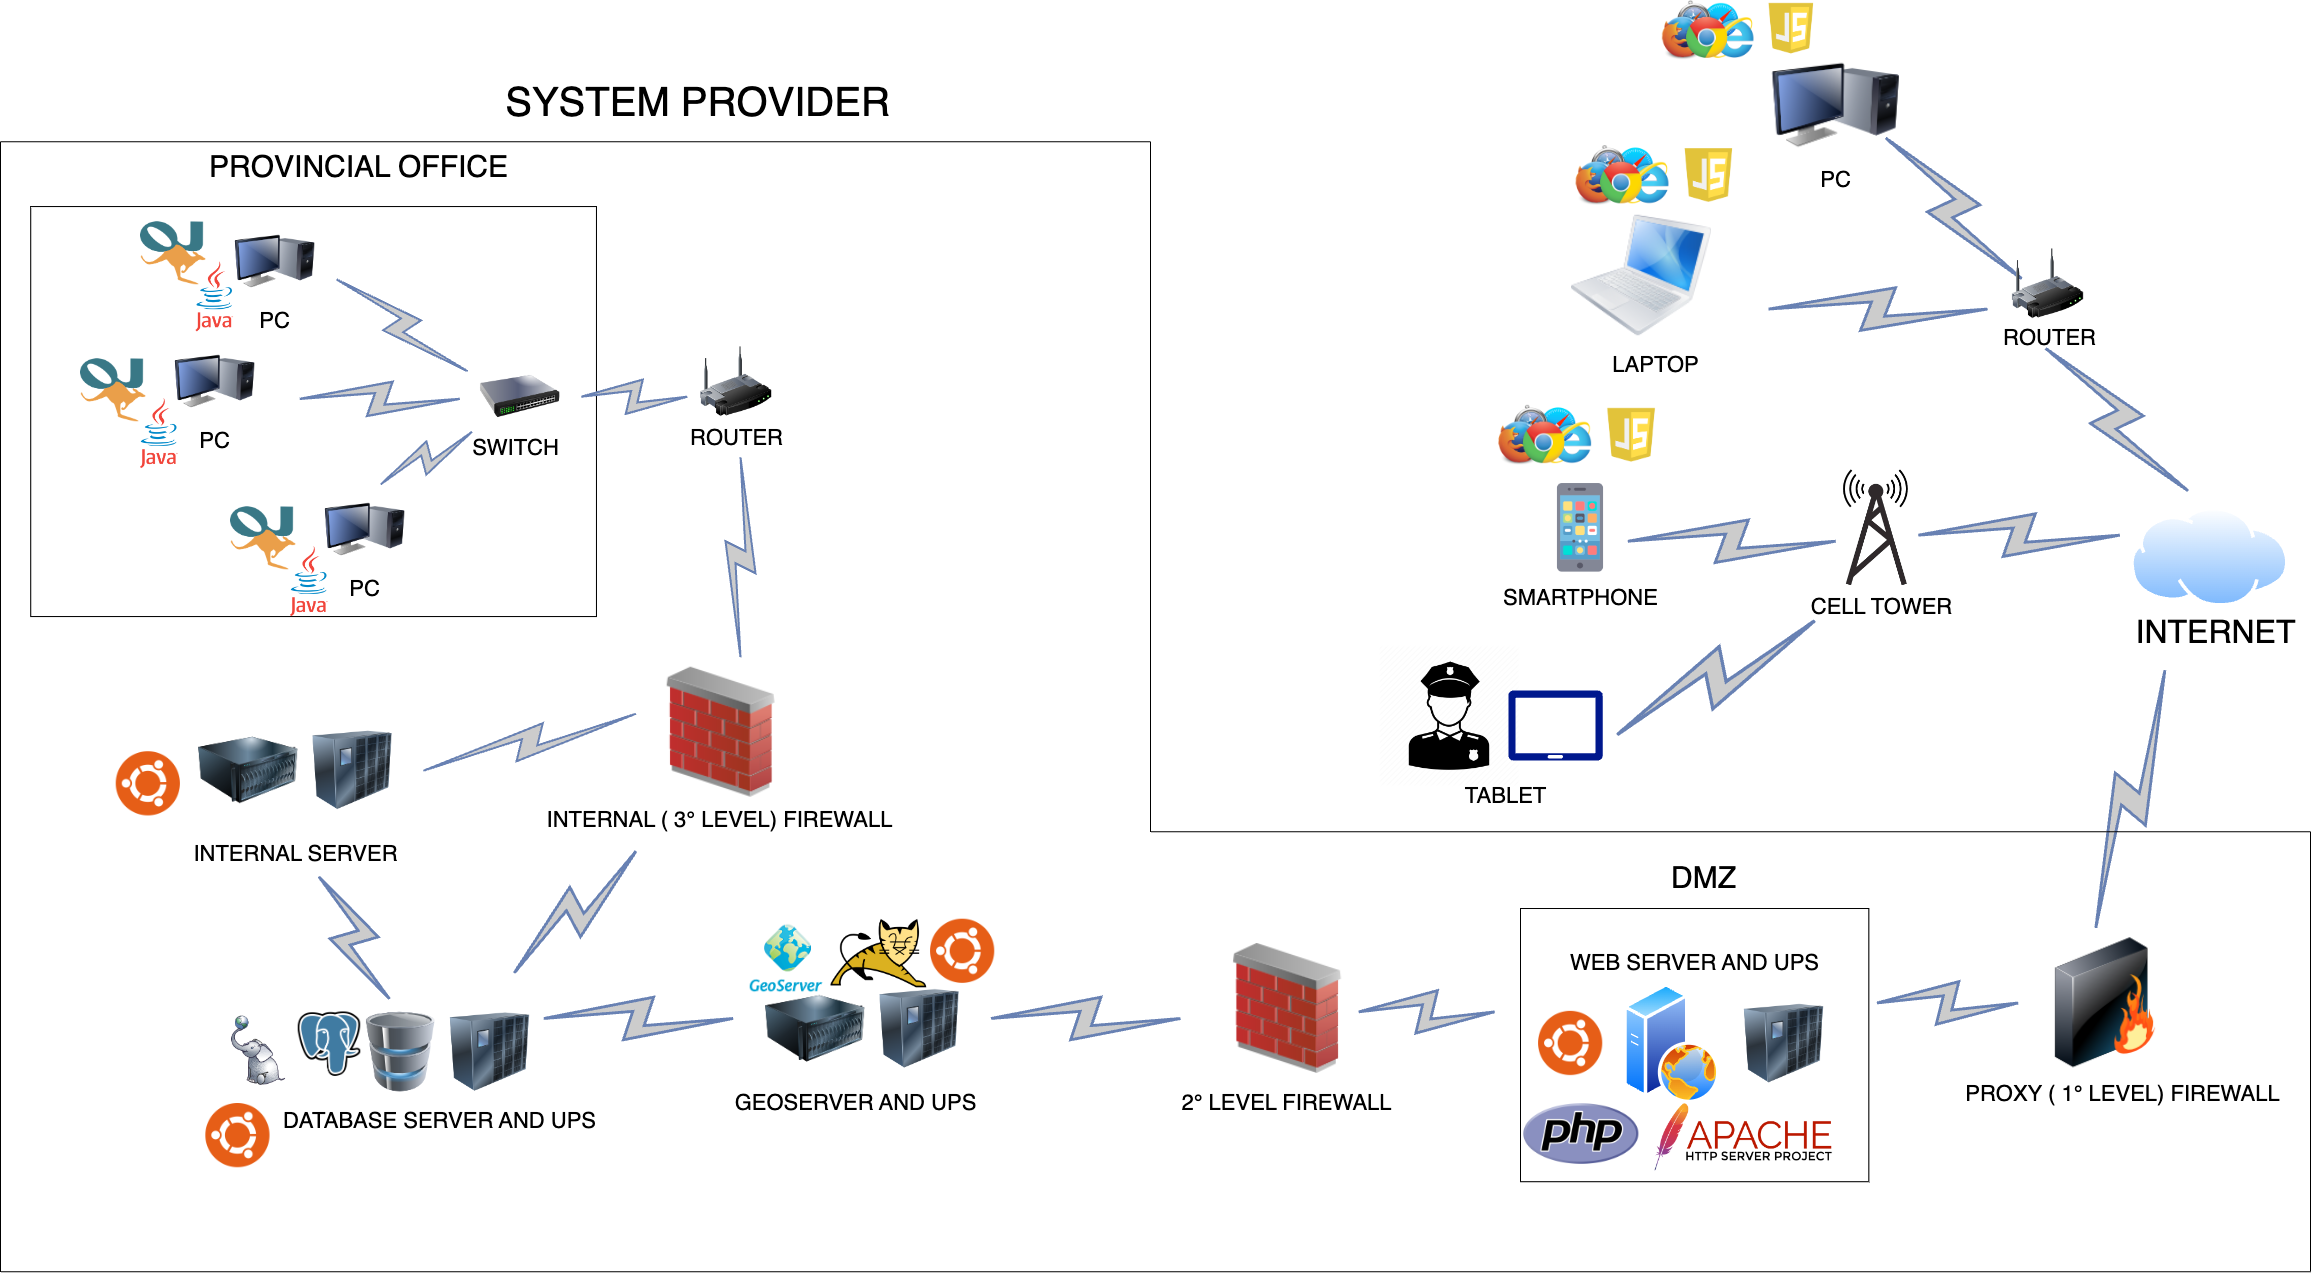
\includegraphics[width=0.7\textwidth]{images/system.png}
        \caption{System schema}
        \label{fig:yourlabel}
       \end{figure}


 Core functionalities of the System:
 \begin{itemize}
     \item \textbf{three level of firewall} for ensuring maximum security. The first level is the proxy firewall to check the incoming connection, the second one handles the access to the GeoServer and Database Server.
     The third one is used internally from the office technicians to access the servers.
     \item \textbf{DMZ} (Demilitarized Zone) is the only area accessible from the public users, hence must be protected by the proxy firewall to ensure "safe" access.
     \item \textbf{UPS} ( Uninterruptible Power Supplies) used to ensure continual power supply to the servers of the System, even when the main power supply fail.
 \end{itemize}

 \subsection{Functionality of the System}
 In this section will be outlined the core functionalites of the Web Application and of the plugins developed for openJUMP.

 \subsubsection{Web Application}
 The Web Application developed is used by the citizens of the Padova municipality for signal the presence of malformations in the road network, and used by the technician of the Provincial office to visualize which reports have been submitted by the citizens. 
 \begin{itemize}
    \newpage
     \item \textbf{HOMEPAGE}
      % \begin{figure}
      %   \centering
      %   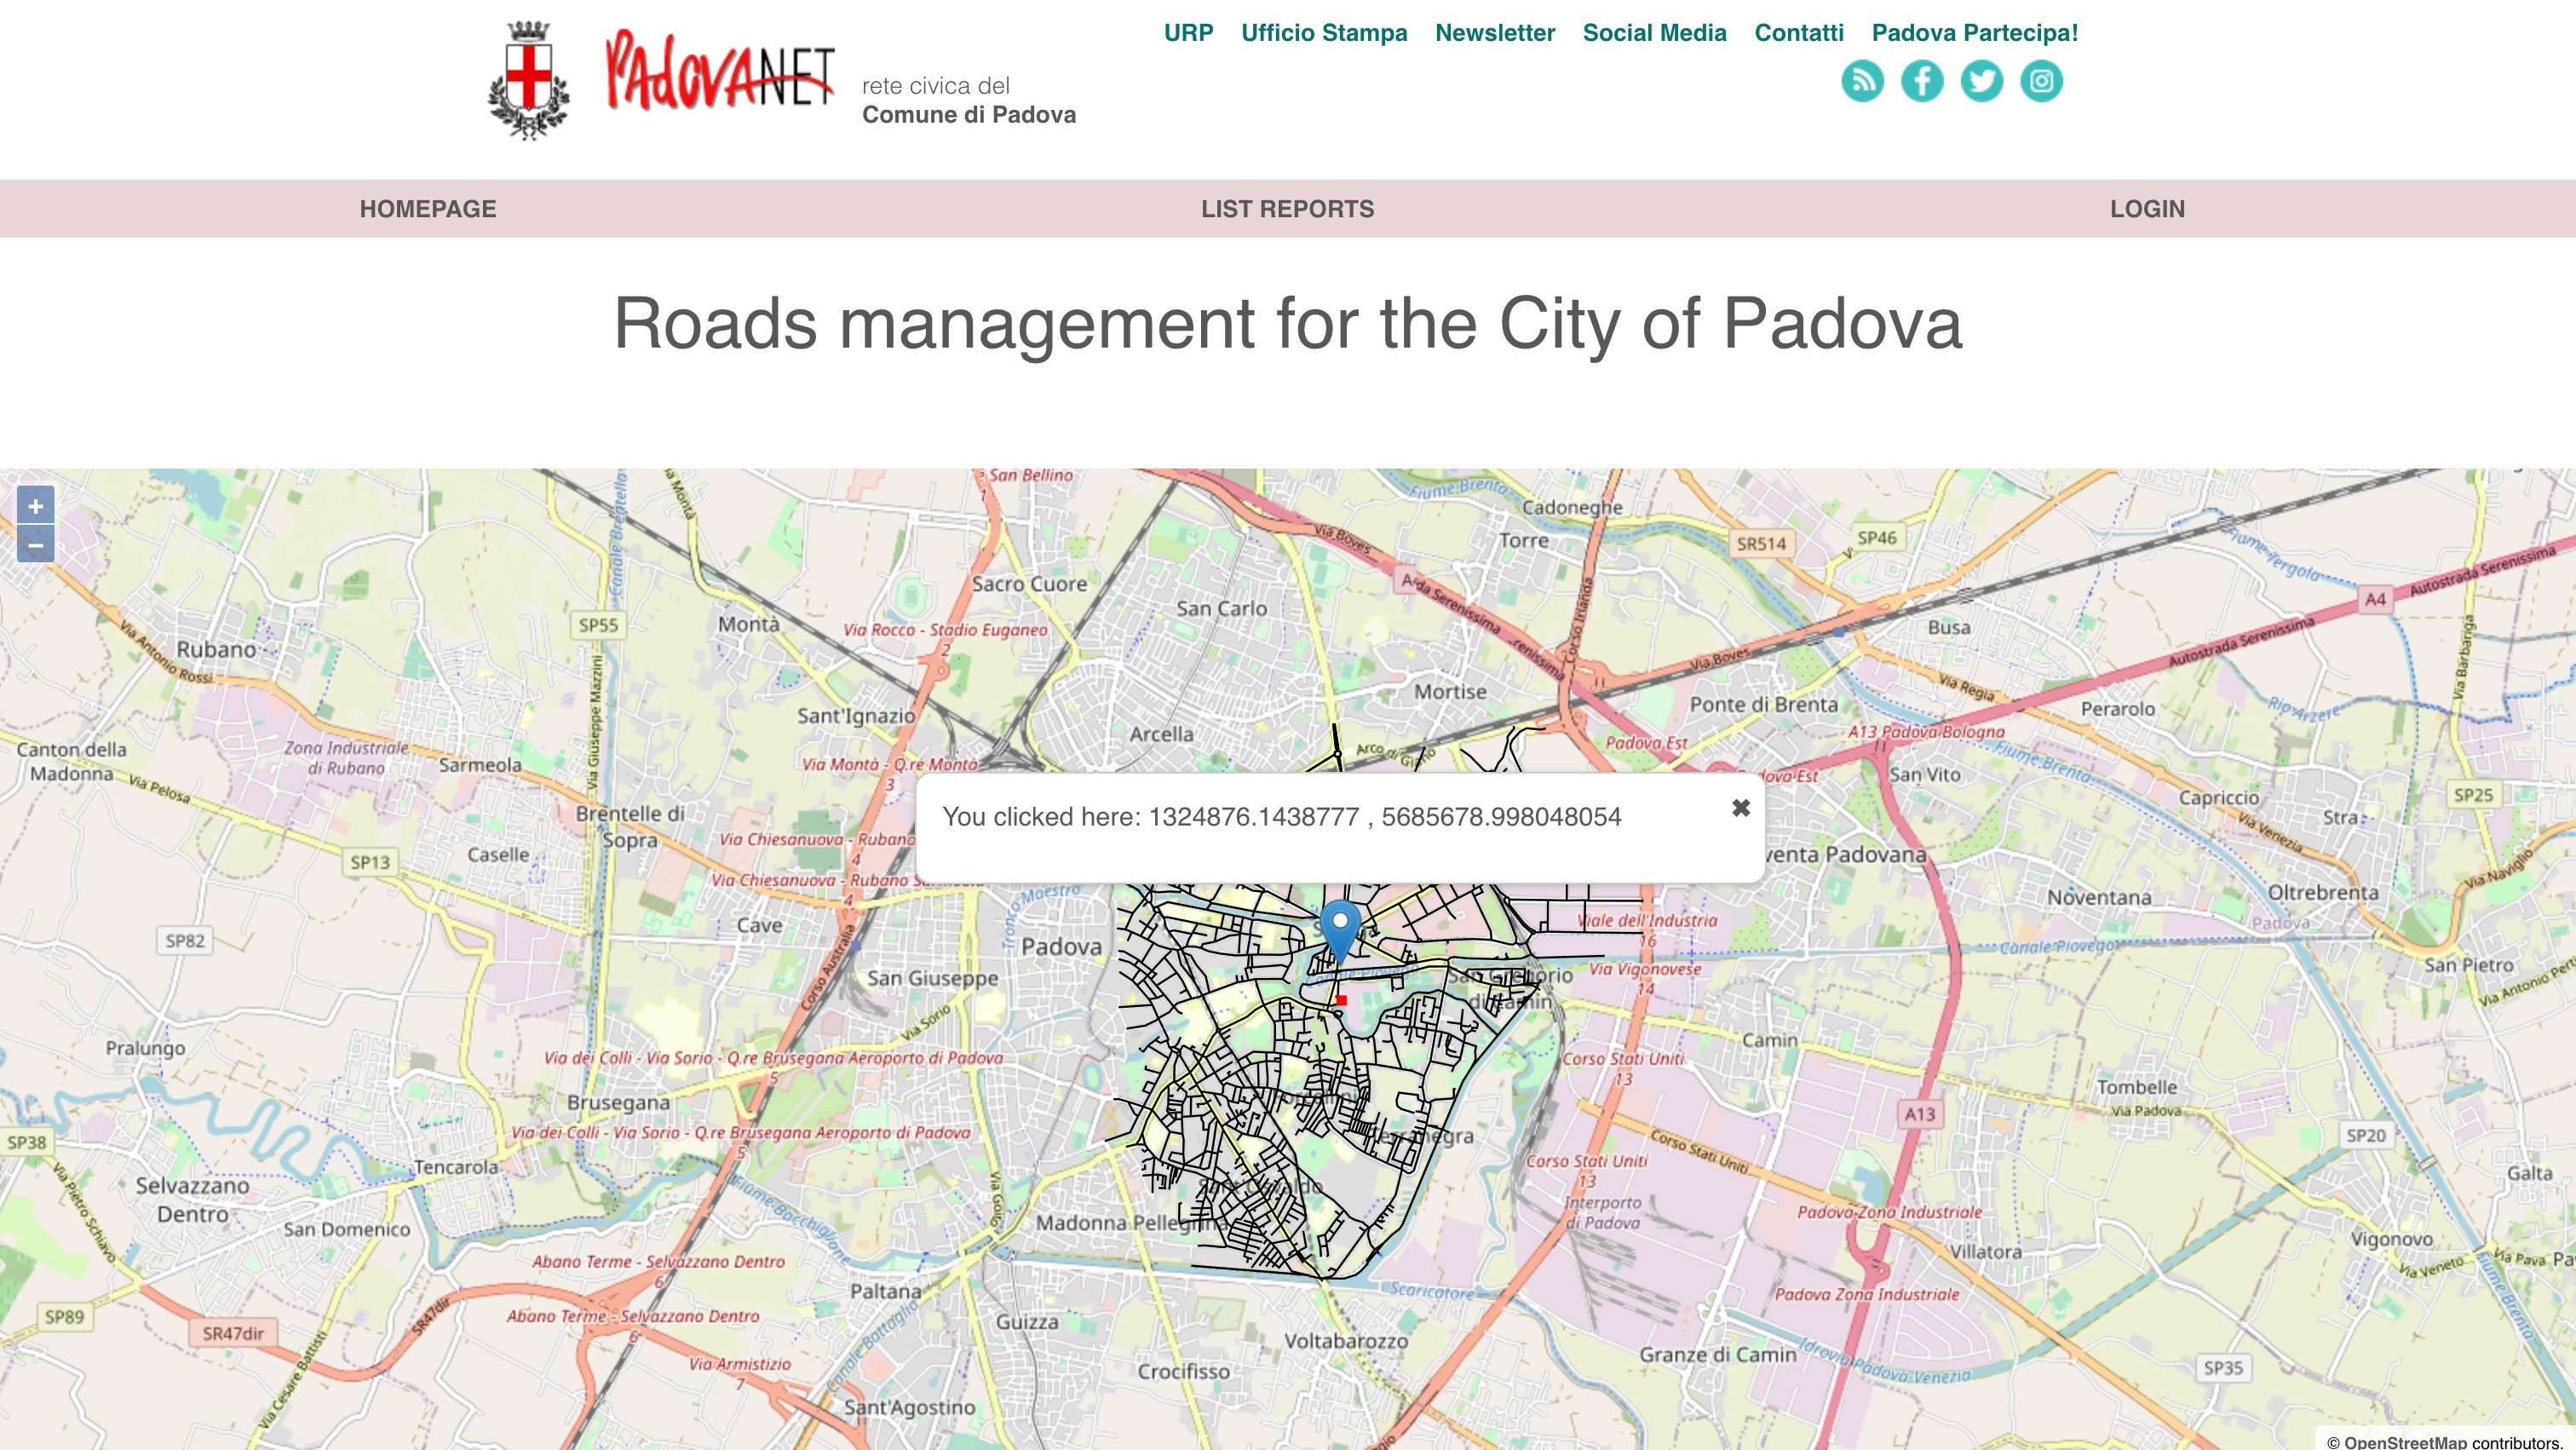
\includegraphics[width=0.7\textwidth]{images/homepage.jpeg}
      %   \caption{Position pin}
      %  \end{figure}
      %  \begin{figure}
      %   \centering
      %   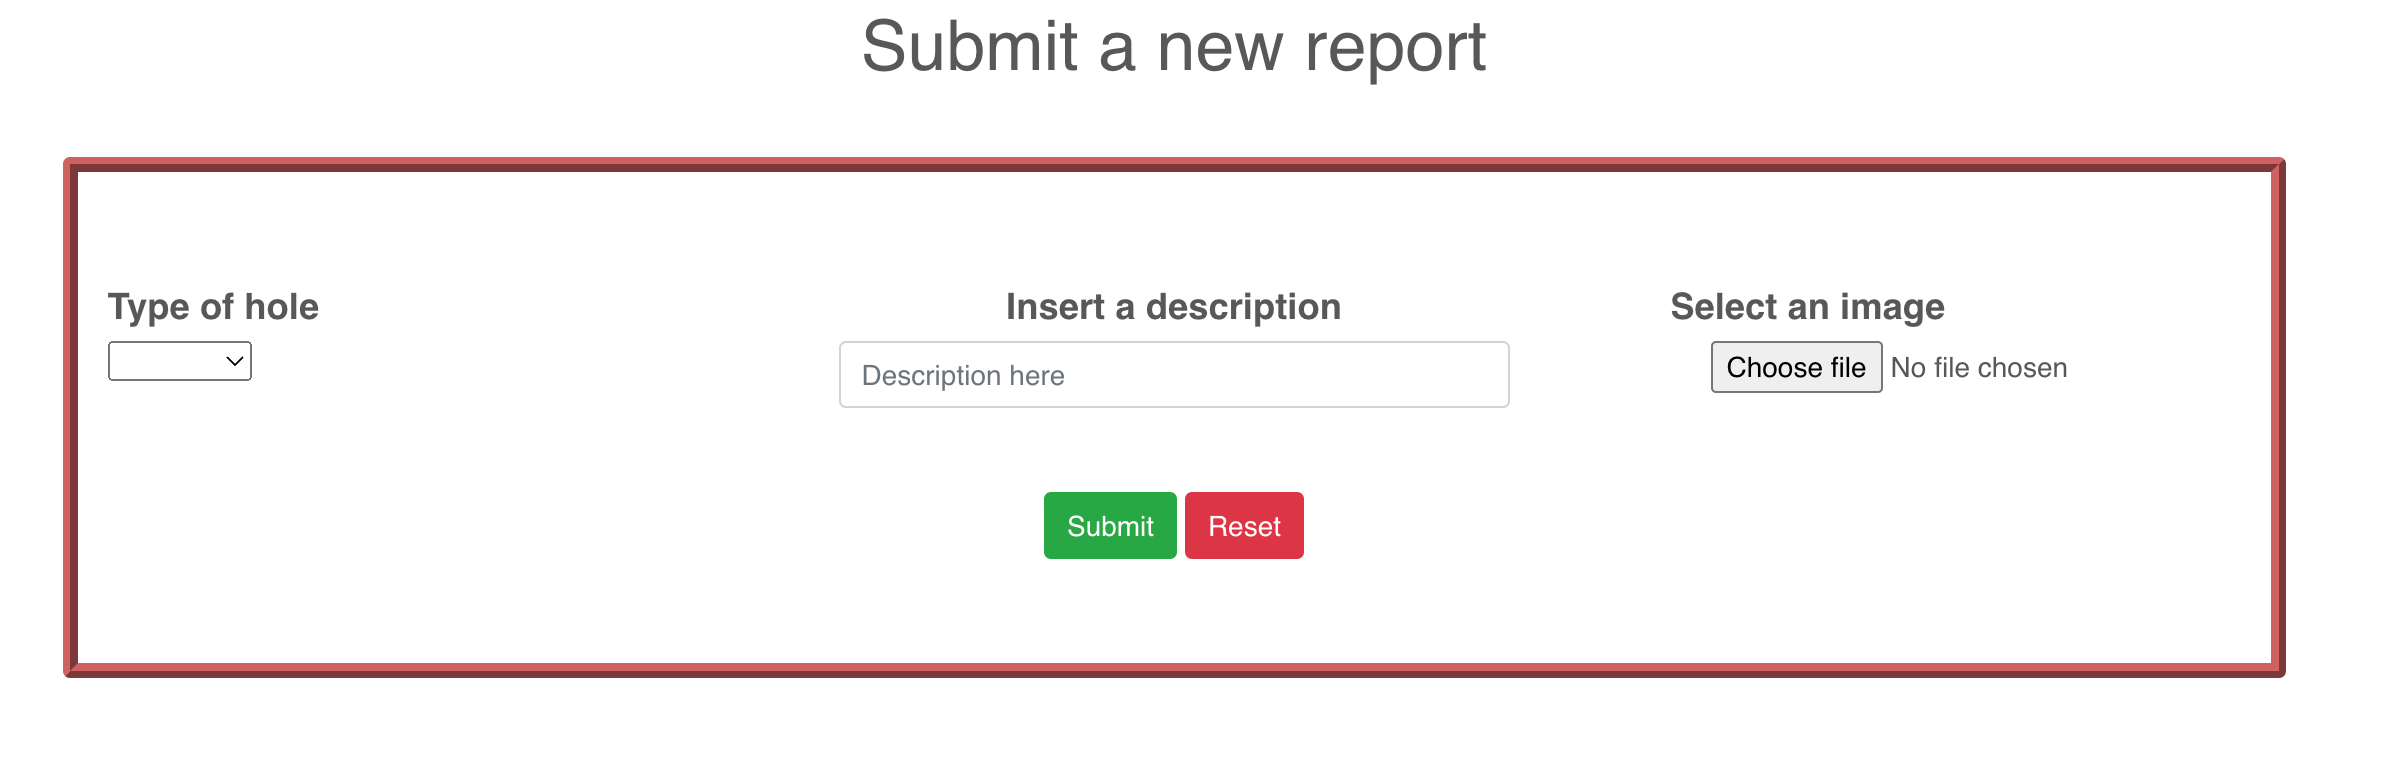
\includegraphics[width=0.7\textwidth]{images/report.png}
      %   \caption{Report form}
      %  \end{figure}

 In the homepage, it is possible to see the map displaying the road network of Padova municipality.
 The user to submit the report must insert the position by clicking on the map or by using the GPS coordinate of the device.
 In the second figure is present the report form for the submission.

    \item \textbf{LOGIN PAGE}
    
    % \begin{figure}
    %     \centering
    %     \centering
    %     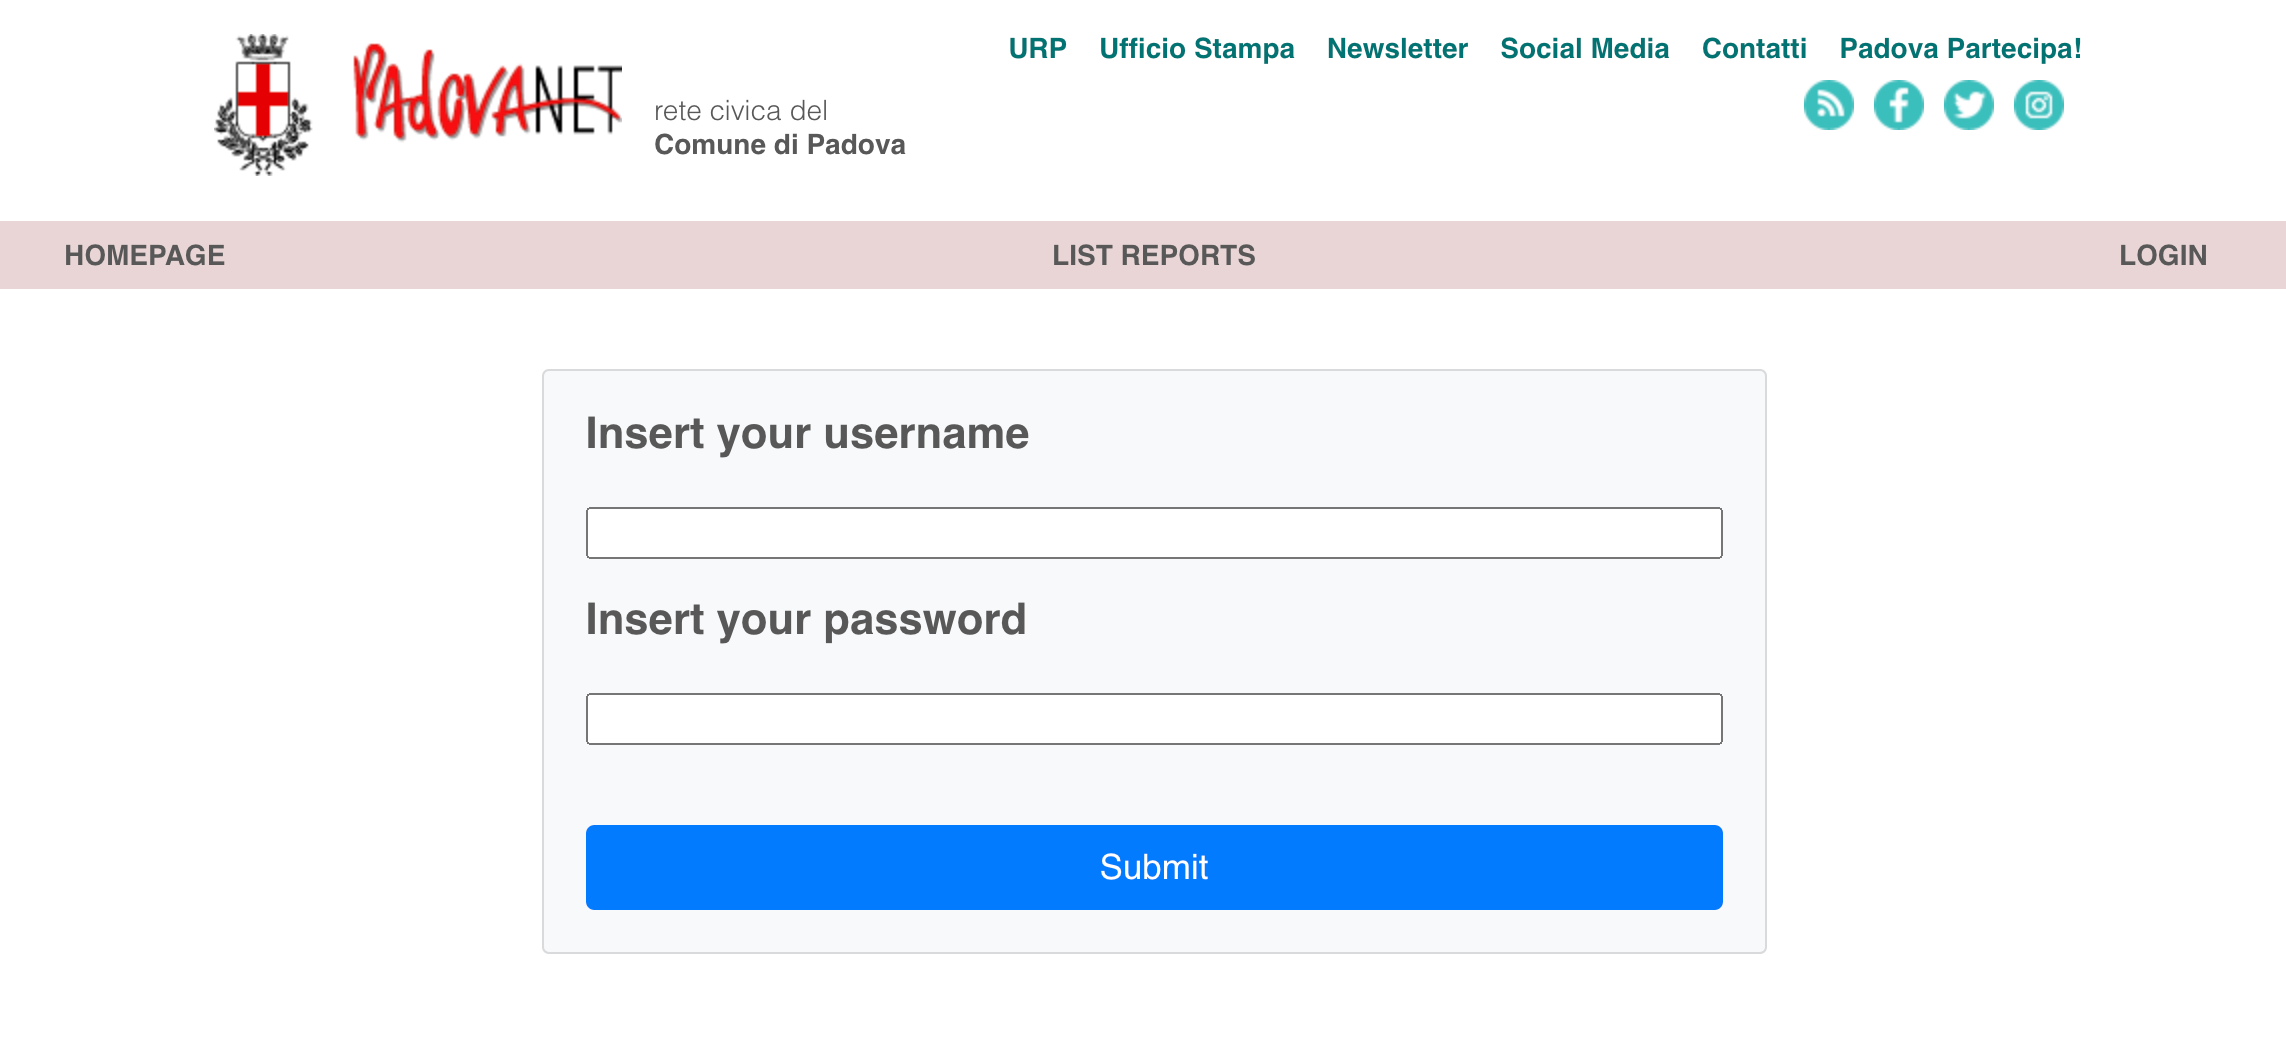
\includegraphics[width=0.7\textwidth]{images/login.png}
    %     \caption{Position pin}
    %     \label{fig:yourlabel}
    % \end{figure}
    To manage unauthorized users, the system is provided of an authentication mechanism made available by the login page; only the technician of the provincial office and the police officers can access to the restricted area by performing the login operation.

    \item \textbf{LIST REPORTS}
    % \begin{figure}
    %     \centering
    %     \centering
    %     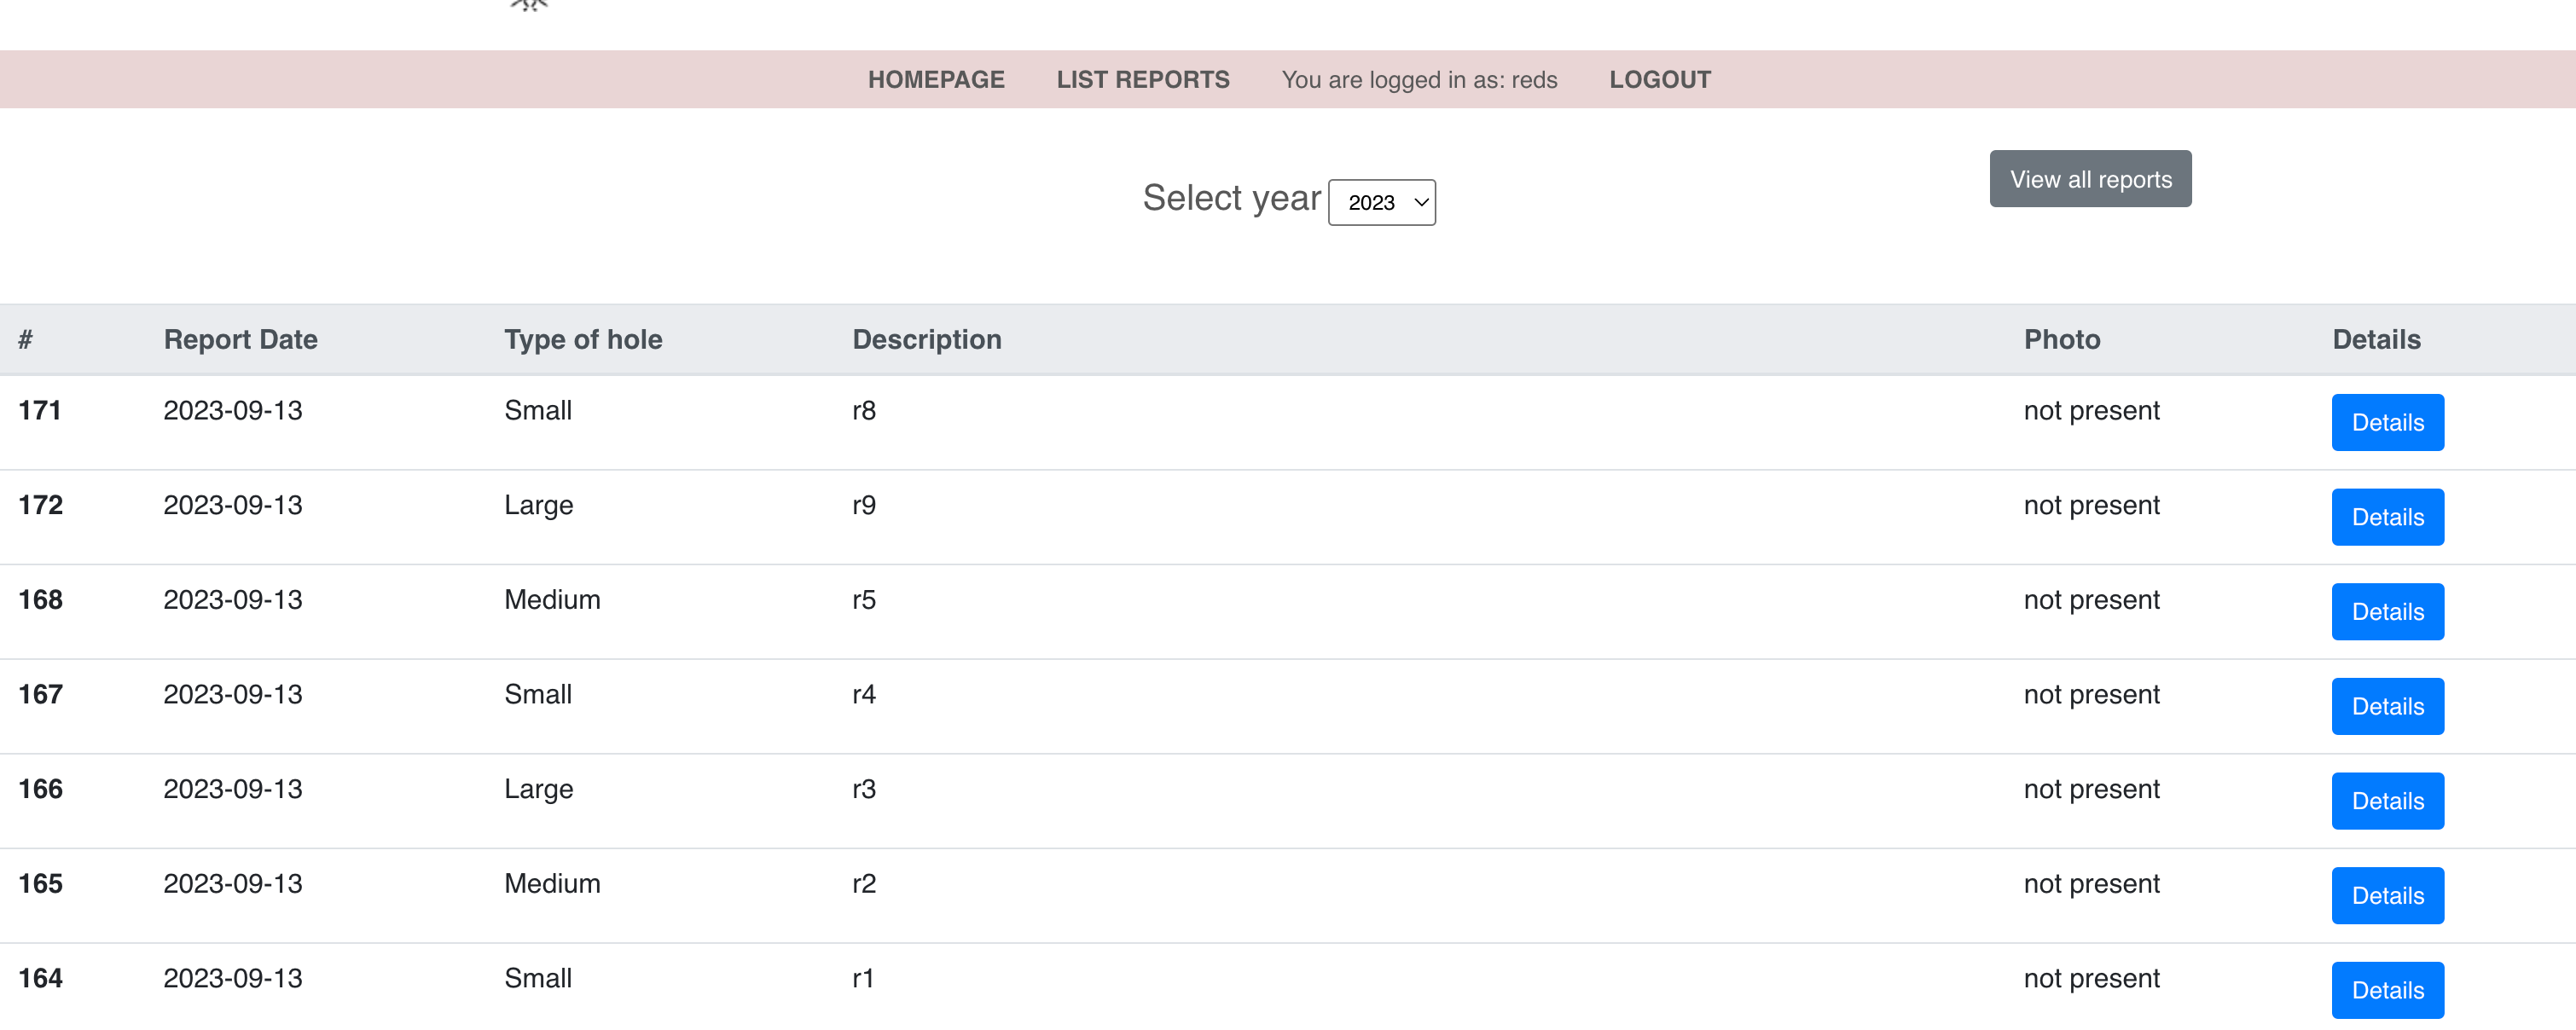
\includegraphics[width=0.7\textwidth]{images/list_reports.png}
    %     \caption{List reports of the selected year}
    %     \label{fig:yourlabel}
    % \end{figure}
    In this restricted area is possible to visualize all report submitted filtered by year. From the page the operator can decide to visualize one or all reports of the selected year.

    \item \textbf{SHOW REPORT}
    % \begin{figure}
    %     \centering
    %     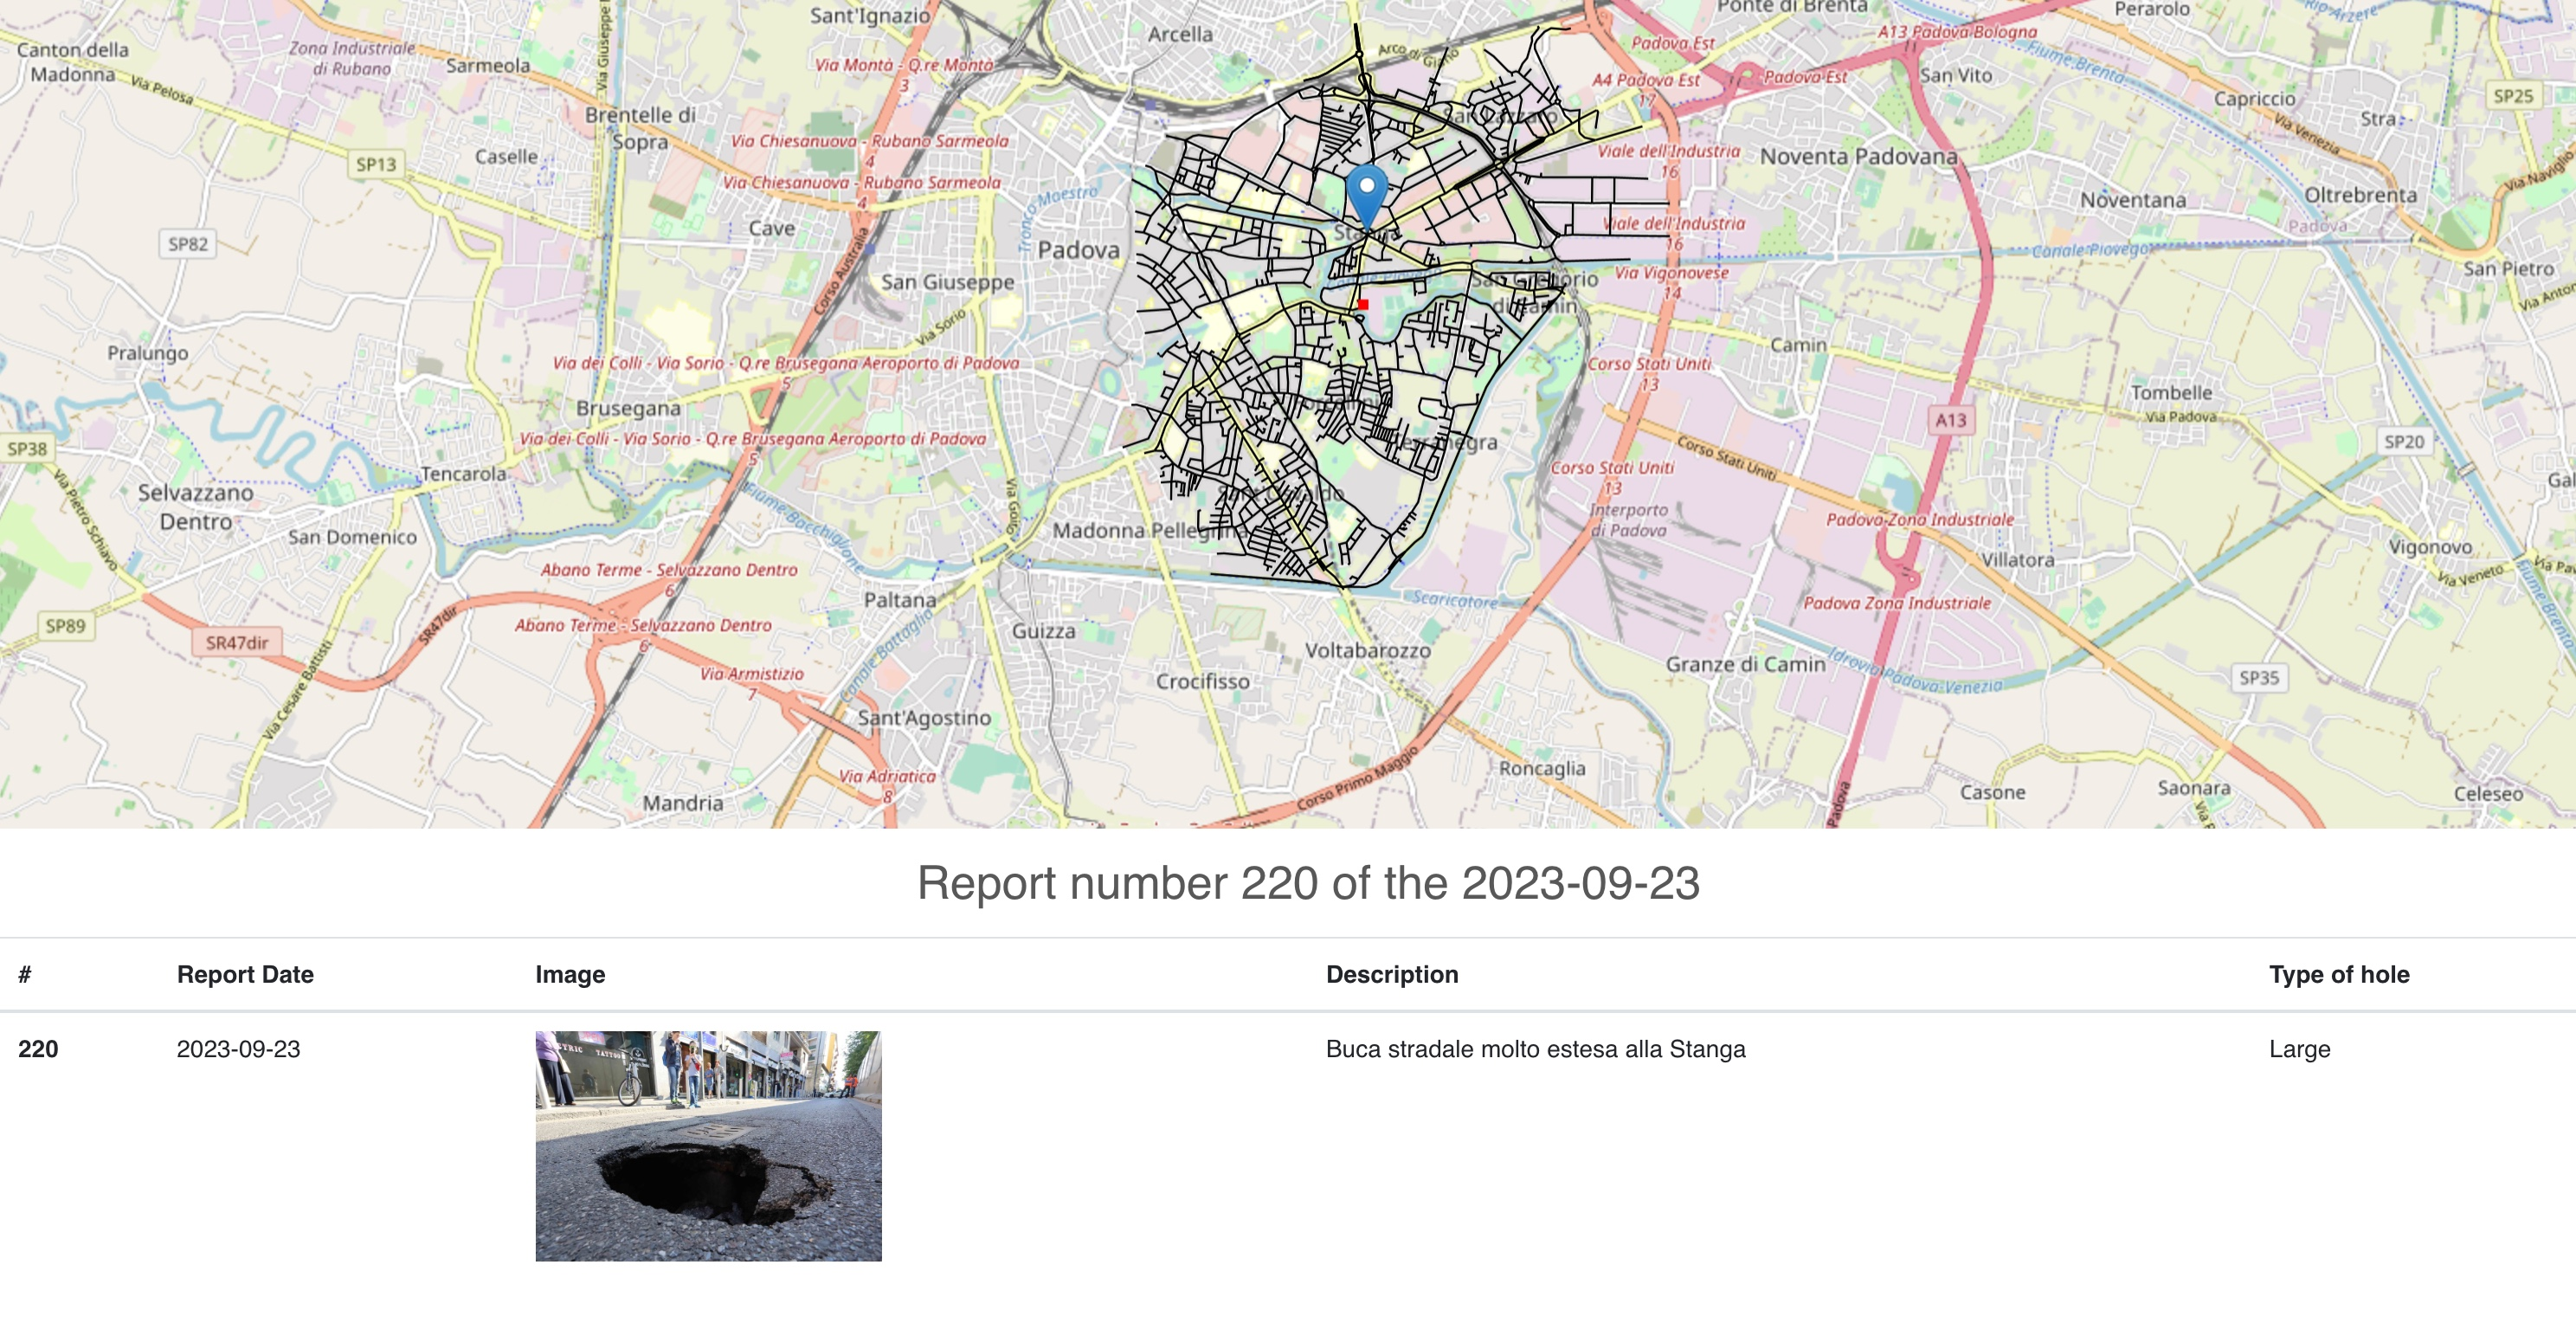
\includegraphics[width=0.7\textwidth]{images/show_report.jpeg}
    %     \caption{Report details}
    %     \label{fig:yourlabel}
    % \end{figure}
    Here it is possible to visualize a specific submitted reports with its positions and all details specified by the citizens in the report.

    \item \textbf{SHOW REPORTS}
    % \begin{figure}
    %     \centering
    %     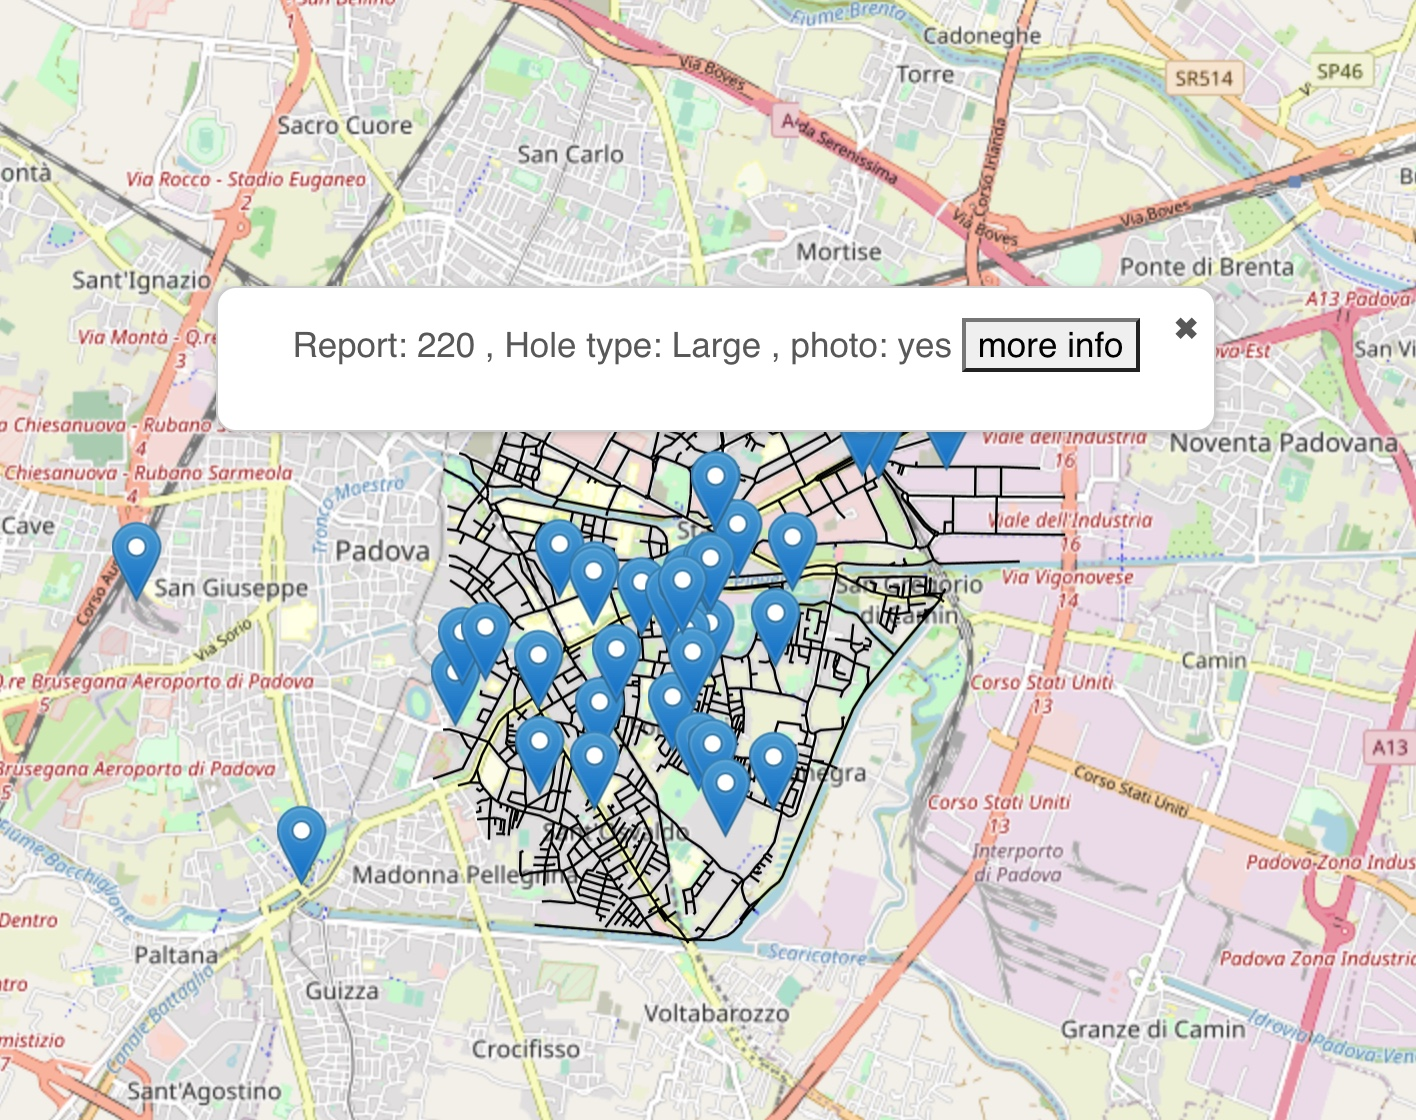
\includegraphics[width=0.7\textwidth]{images/show_reports.jpeg}
    %     \caption{Pins of all reports of the specified year}
    %     \label{fig:yourlabel}
    % \end{figure}
    In the show reports page we can see all the submitted reports for the specified year, as a pin in the map. By clicking on the marker it is possible to see a short preview of the report, and by clicking the button to go to the show report page to get full informations about that report.
\end{itemize}

 \subsubsection{openJUMP plugins}

 \subsection{Database}
 \subsubsection{ER Schema}
 \subsubsection{Description of the Entities and the Relationship of the ER Schema}